\documentclass[tikz,border=4pt]{standalone}
\usepackage{tikz}
\usepackage{amsmath}
\usetikzlibrary{calc,arrows.meta,positioning,shapes.geometric}

\begin{document}
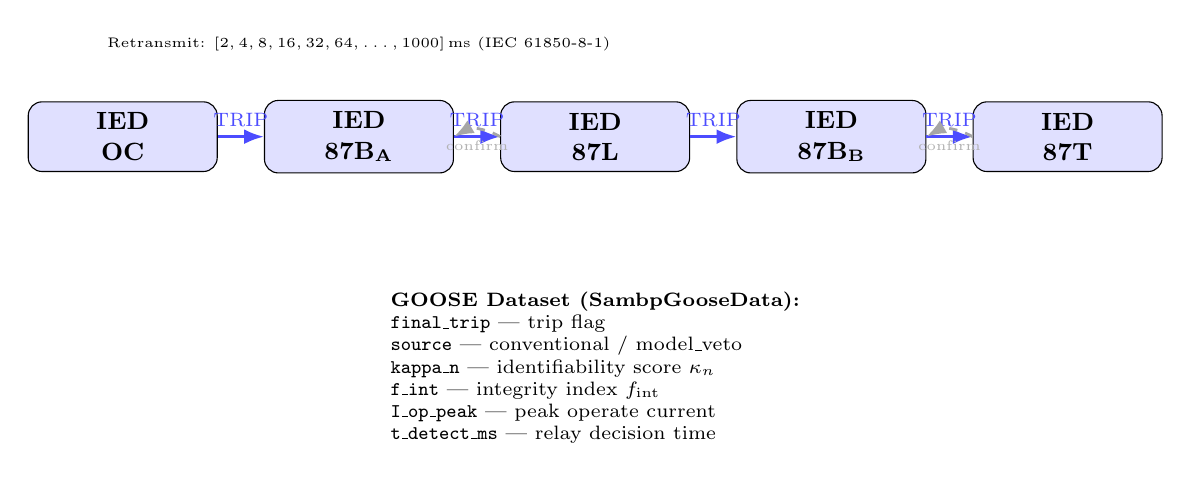
\begin{tikzpicture}[
    ied/.style={draw,fill=blue!12,rounded corners=5pt,
                minimum width=2.4cm,minimum height=0.85cm,
                font=\small\bfseries,align=center,inner sep=4pt},
    goose/.style={-{Latex[length=2.5mm]},line width=1.0pt,blue!70},
    goose2/.style={-{Latex[length=2.5mm]},line width=1.0pt,
                   dashed,gray!70},
    label/.style={font=\scriptsize,text=blue!70},
    ann/.style={font=\tiny,text=gray!60},
]

% IEDs in a row
\node[ied] (OC)   at (0,0)    {IED\\ OC};
\node[ied] (BA)   at (3,0)    {IED\\ 87B\textsubscript{A}};
\node[ied] (L)    at (6,0)    {IED\\ 87L};
\node[ied] (BB)   at (9,0)    {IED\\ 87B\textsubscript{B}};
\node[ied] (T)    at (12,0)   {IED\\ 87T};

% Forward GOOSE (zone acceleration)
\draw[goose] (OC.east)  -- node[above,label]{TRIP}  (BA.west);
\draw[goose] (BA.east)  -- node[above,label]{TRIP}  (L.west);
\draw[goose] (L.east)   -- node[above,label]{TRIP}  (BB.west);
\draw[goose] (BB.east)  -- node[above,label]{TRIP}  (T.west);

% Reverse GOOSE (zone confirmation)
\draw[goose2] (T.west)  to[bend right=30]
              node[below,ann]{confirm} (BB.east);
\draw[goose2] (L.west)  to[bend right=30]
              node[below,ann]{confirm} (BA.east);

% SAMBP state in dataset
\node[font=\scriptsize,align=left,
      below=1.1cm of L.south,yshift=-0.3cm]
    {\textbf{GOOSE Dataset (SambpGooseData):}\\
     \texttt{final\_trip} — trip flag\\
     \texttt{source} — conventional / model\_veto\\
     \texttt{kappa\_n} — identifiability score $\kappa_n$\\
     \texttt{f\_int} — integrity index $f_{\rm int}$\\
     \texttt{I\_op\_peak} — peak operate current\\
     \texttt{t\_detect\_ms} — relay decision time};

% Retransmission annotation
\node[font=\tiny,align=left,above=0.5cm of BA.north]
    {Retransmit: $[2,4,8,16,32,64,\ldots,1000]$\,ms (IEC~61850-8-1)};

\end{tikzpicture}
\end{document}
